\documentclass{standalone}
\usepackage{tikz}
\usetikzlibrary{circuits.logic.US,shapes.gates.logic.IEC}
\tikzstyle{branch}=[fill,shape=circle,minimum size=2pt,inner sep=0pt]
\begin{document}
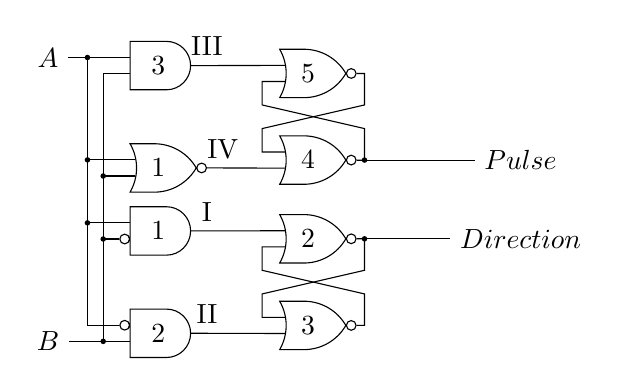
\begin{tikzpicture}[circuit logic US]
\node (A) at (0,1.8) {$A$};
\node (B) at (0,-1.8) {$B$};
\node[and gate, draw, inputs=ni] at ($(1.4,-0.4)$) (And1) {1};
\node[and gate, draw, inputs=in] at ($(1.4,-1.7)$) (And2) {2};
\node[and gate, draw, inputs=nn] at ($(1.4,+1.7)$) (And3) {3};
\node[nor gate, draw, inputs=nn] at ($(1.4,+0.4)$) (Nor1) {1};
\node[nor gate, draw, inputs=nn] at ($(And1) +(1.9,-0.1)$) (Nor2) {2};
\node[nor gate, draw, inputs=nn] at ($(And2) +(1.9,+0.1)$) (Nor3) {3};
\node[nor gate, draw, inputs=nn] at ($(Nor1) +(1.9,+0.1)$) (Nor4) {4};
\node[nor gate, draw, inputs=nn] at ($(And3) +(1.9,-0.1)$) (Nor5) {5};
\node (P) at ($(Nor4)+(2.7,0)$) {$Pulse$};
\node (D) at ($(Nor2)+(2.7,0)$) {$Direction$};
\draw (A) -- +(0.5,0) |- node[branch]{} (And1.input 1);
\draw (B) -- +(0.7,0) |- node[branch]{} (And1.input 2);
\draw (A) -- +(0.5,0) |- (And2.input 1);
\draw (B) -- +(0.7,0) |- node[branch]{} (And2.input 2);
\draw (A) -- +(0.5,0) |- node[branch]{} (And3.input 1);
\draw (B) -- +(0.7,0) |- (And3.input 2);
\draw (A) -- +(0.5,0) |- node[branch]{} (Nor1.input 1);
\draw (B) -- +(0.7,0) |- node[branch]{} (Nor1.input 2);
\draw (And1.output) -- +(0.2,0) node[above]{I} -- (Nor2.input 1);
\draw (And2.output) -- +(0.2,0) node[above]{II} -- (Nor3.input 2);
\draw (Nor2.output) -| node[branch]{} +(0.1,-0.4) -- +(-1.2,-0.7) |- (Nor3.input 1);
\draw (Nor3.output) -| +(0.1,0.4) -- +(-1.2,0.7) |- (Nor2.input 2);
\draw (Nor2.output) -- (D);
\draw (And3.output) -- +(0.2,0) node[above]{III} -- (Nor5.input 1);
\draw (Nor1.output) -- +(0.2,0) node[above]{IV} -- (Nor4.input 2);
\draw (Nor5.output) -| +(0.1,-0.4) -- +(-1.2,-0.7) |- (Nor4.input 1);
\draw (Nor4.output) -| node[branch]{} +(0.1,0.4) -- +(-1.2,0.7) |- (Nor5.input 2);
\draw (Nor4.output) -- (P);
\end{tikzpicture}
\end{document}
